\documentclass[12pt,a4paper]{article}

% Margins.
\setlength{\oddsidemargin}{0in}
\setlength{\evensidemargin}{0in}
\setlength{\headheight}{12pt}
\setlength{\headsep}{42pt}
\setlength{\topmargin}{-54pt}
\setlength{\textwidth}{6.5in}
\setlength{\textheight}{10in}

\usepackage{amsmath}
\usepackage{float}
\usepackage{graphicx}
\usepackage[hyphens]{url}
\usepackage{hyperref}	% Clickable links to figures, references and urls.
\usepackage{datetime}
\usepackage{longtable}
\usepackage{subfigure}

% Links direct to top of figures.
\usepackage[all]{hypcap}

% Drawing.
\usepackage{pgf}
\usepackage{tikz}

% Listings for formatting code.
\usepackage{listings}
\usepackage{textcomp}
% General options.+++
\lstset{breaklines=true, basicstyle=\small\ttfamily, tabsize=4, numbers=left, stepnumber=1, frame=single, showstringspaces=false, upquote=true}
% C++ specific high-lighting. Comments are 50/50 shades of green/black and strings coloured with 60/40 red/black mixture.
\lstset{language=[ISO]C++, commentstyle=\color{green!50!black}, keywordstyle=\color{blue}, stringstyle=\color{red!60!black}}

%opening
\title{\vspace{-3cm}Physics for Engineers\\Class 28\\Electric Potential of Point Charge}
\author{Attique Dawood}
\date{March 27, 2014\\[0.2cm] Last Modified: \today, \currenttime}
\begin{document}
\maketitle
\section{Announcements}
\begin{itemize}
\item None.
\end{itemize}
\section{Revision}
Work done in moving a charge $q$ from A to B in an electric field \textbf{E} is
\begin{equation}
W_{AB}=-q\int\limits_{A}^{B} \textbf{E}\cdot d\textbf{\textit{l}}.
\end{equation}
If an electric field exists in a region then electric potential between two points, A and B, is
\begin{equation}
V_{AB}=V_B-V_A=-\int\limits_{A}^{B} \textbf{E}\cdot d\textbf{\textit{l}}.
\end{equation}
Absolute electric potential at a point B is
\begin{equation}
V_{B}=-\int\limits_{\infty}^{B} \textbf{E}\cdot d\textbf{\textit{l}}.
\end{equation}
Absolute potential field of a point charge $q$ at origin is
\begin{equation}
V(\textbf{r})=\dfrac{q}{4\pi\epsilon_0r}.
\end{equation}
If the point charge is located at $\textbf{r}'$ then potential field is
\begin{equation}
V(\textbf{r})=\dfrac{q}{4\pi\epsilon_0|\textbf{r}-\textbf{r}'|}.
\end{equation}
\section{Energy of System of Charges}
We have discussed electric field due to arrangement of point charges and continuous charge distributions. To bring similar charges together we need to some work. We are now interested in the amount of energy or work that must be done to bring together a bunch of charges.

Suppose we have a charge $q_1$. We bring this charge from infinity and place it at $r_1'$. How much work was done? Since, there was no electric field, total work done is $W_1=0$. We take another charge $q_2$, bring it from infinity and place at $r_2'$. How much work is done? If we know the absolute potential, $V_2$, at $r_2'$ due to $q_1$ we can simply multiply $q_2$ with $V_2$ to find the work done. Given distance between $q_1$ and $q_2$ as $r_{12}$ the electric potential of $q_1$ at $r_2'$ is
\begin{equation}
V_2=\dfrac{q_1}{4\pi\epsilon_0r_{12}}.
\end{equation}
Work done in moving $q_2$ from infinity to $r_2'$ is then
\begin{equation}
W_2=q_2V_2=\dfrac{q_1q_2}{4\pi\epsilon_0r_{12}}.
\end{equation}
We take another charge $q_3$, bring it from infinity and place at $r_3'$. Since, we have to move this charge against the electric fields of both $q_1$ and $q_2$ total work done is given by
\begin{equation}
W_3=q_3V_3=\dfrac{q_1q_3}{4\pi\epsilon_0r_{13}}+\dfrac{q_2q_3}{4\pi\epsilon_0r_{23}}.
\end{equation}
Here is $V_3$ is the absolute potential at $r_3'$ due to $q_1$ and $q_2$.
\begin{equation}
V_3=\dfrac{q_1}{4\pi\epsilon_0r_{13}}+\dfrac{q_2}{4\pi\epsilon_0r_{23}}.
\end{equation}
The total work done in assembling these three charges is
\begin{equation}
W=W_1+W_2+W_3=0+\dfrac{q_1q_2}{4\pi\epsilon_0r_{12}}+\dfrac{q_1q_3}{4\pi\epsilon_0r_{13}}+\dfrac{q_2q_3}{4\pi\epsilon_0r_{23}}.
\end{equation}
Or
\begin{equation}
W=\dfrac{q_1q_2}{4\pi\epsilon_0r_{12}}+\dfrac{q_2q_3}{4\pi\epsilon_0r_{23}}+\dfrac{q_3q_1}{4\pi\epsilon_0r_{31}}.
\end{equation}
\section{Exercises}
\noindent\textbf{Question 1:} A 1 C charge is located at origin.
\begin{itemize}
\item[a.] Find electric potential, $V_A$ at point A(1, 1, 1).
\item[b.] Find electric potential, $V_B$ at point B(1, 1, 2).
\item[c.] Calculate the potential difference $V_{AB}$ between A and B.
\item[d.] Calculate the work done in moving a 2 C charge from A to B.
\end{itemize}
\noindent\textbf{Question 2:} A 1 C charge is located at (1, 0, 0) and a -1 C charge is located at (0, 1, 0).
\begin{itemize}
\item[a.] Find electric potential at point A(1, 1, 0).
\item[b.] Find electric potential at point B(3, 1, 2).
\end{itemize}
%\begin{itemize}
%\item[a.] Electric field of a point charge.
%\item[b.] Electric field of an infinite line charge placed along $z$--axis.
%\end{itemize}
%%\begin{figure}[H]
%\centering
%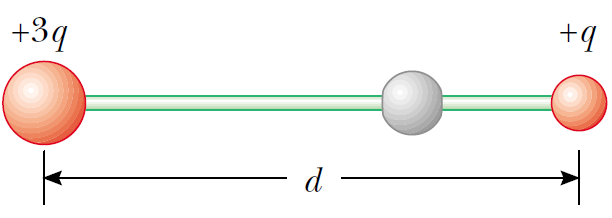
\includegraphics[scale=0.45]{FigureP23-10.png}
%\caption{Equilibrium of charge.}
%\label{Equilibrium}
%\end{figure}
%\nocite{*}
%\bibliographystyle{plain}
%\bibliography{PhysicsRef}
\end{document}
